
%
%  $Description: Author guidelines and sample document in LaTeX 2.09$
%
%  $Author: ienne $
%  $Date: 1995/09/15 15:20:59 $
%  $Revision: 1.4 $
%

\documentclass[times, 10pt,twocolumn]{article}
\usepackage{latex8}
\usepackage{times}
%my packages:
\usepackage{graphicx}
\usepackage{amsmath}
\usepackage{amssymb}


%\documentstyle[times,art10,twocolumn,latex8]{article}

%-------------------------------------------------------------------------
% take the % away on next line to produce the final camera-ready version
\pagestyle{empty}

%-------------------------------------------------------------------------
\begin{document}

\title{SMT-based Test Program Generation for Cache-memory Testing}

\author{Evgeni Kornikhin\\
Institute for System Programming of RAS\\ Solzhenitsyn St., 25, Moscow, Russia\\ kornevgen@ispras.ru\\
}

\maketitle
\thispagestyle{empty}

\begin{abstract}
Core-level verification of microprocessors is performed using
many assembly programs (test programs). Instructions (and their behavior) for test program can be selected combinatorially. But special initial values for registers are required to satisfy this test program. This article proposes algorithm for generation these values. The article considers instructions performed memory access through cache. Proposing algorithm describes test program behavior as SMT-assertions and uses SMT-solvers to get initial values of registers for given initial state of cache-memory.
\end{abstract}



\section{Introduction}

System functional testing of microprocessors uses many assembly
programs (\emph{test programs}). Such programs are loaded to the
memory, executed, execution process is logged and analyzed. But
modern processors testing requires a lot of test programs. Technical
way of test program generation was proposed in~\cite{kamkin}. This
way based on the microprocessor's model. Its first stage is
systematic generation abstract test programs (\emph{test
templates}). This abstract form contains a sequence of instructions
with arguments (registers) and \emph{test situations} (behavior of
this instruction; these can be overflow, cache hits, cache misses).
The second stage is generation of initial microprocessor state for
given test template, i.e. initial values of registers. Technical way
from~\cite{kamkin} is useful for aimed testing when aim is expressed
by instruction sequence with specific behavior. Based on registers
values the third, final, stage is generation the sequence of
instructions to reach initial microprocessor state. This sequence of
instructions with test template get ready assembly program. This
paper devoted to the second stage, i.e. initial state generation.

Known researches about test data generation problem contain the
following methods of its solving:
\begin{enumerate}
\item combinatorial methods;
\item ATPG-based methods;
\item constraint-based methods.
\end{enumerate}

Combinatorial methods are useful for simple test templates (each
variable has explicit directive of its domain, each value in domain
is possess)~\cite{combinatorial}. ATPG-based methods are useful for
structural but not functional testing~\cite{ATPG}. Constraint-based
methods are the most promising methods. Test template is translated
to the set of constraints (predicates) with variables which
represented test data. Then special solver generates values for
variables to satisfy all constraints. This paper contains
constraint-based method also. IBM uses constraint-based method in
Genesys-Pro~\cite{GenesysPro}. But it works inefficiently on test
templates from~\cite{kamkin}. Authors of another constraint-based
methods restrict on registers only and don't consider cache-memory.

\section{Preliminaries}

\subsection{Test templates description}

Test template defines requirements to the future test program. Test
template contains sequence of instructions. Each element of this
sequence has instruction name, arguments (registers, addresses,
values) and \emph{test situation} (constraint on values of arguments and
microprocessor state before execution of instruction). Example of
test template description for model instruction set:

REGISTER reg1 : 32;

REGISTER reg2 : 32;

LOAD reg1, reg2 @ l1Miss

STORE reg2, reg1 @ l1Hit

This template has 2 instructions -- LOAD and STORE. Template
begins from variable definitions (consist of name and bit-length). Test situation is specified after "@": test situation
of the first instruction if "l1Hit" (which means hit in first-level cache) and test situation of the second instruction is "l1Miss" (which means miss in first-level cache).

\begin{itemize}
\item "LOAD reg1, reg2" loads value from memory by \emph{virtual} address from register "reg2" to the register "reg1";
\item "STORE reg1, reg2" stores value from register "reg1" to the
memory by \emph{virtual} address in "reg2".
\end{itemize}

Behavior of "LOAD/STORE x, y" is the following: the first step is
physical address generation (\emph{address translation}) and the
second step is memory access through cache using generated physical address (see pic.~\ref{LOAD}).

\begin{figure}[h]\label{LOAD}
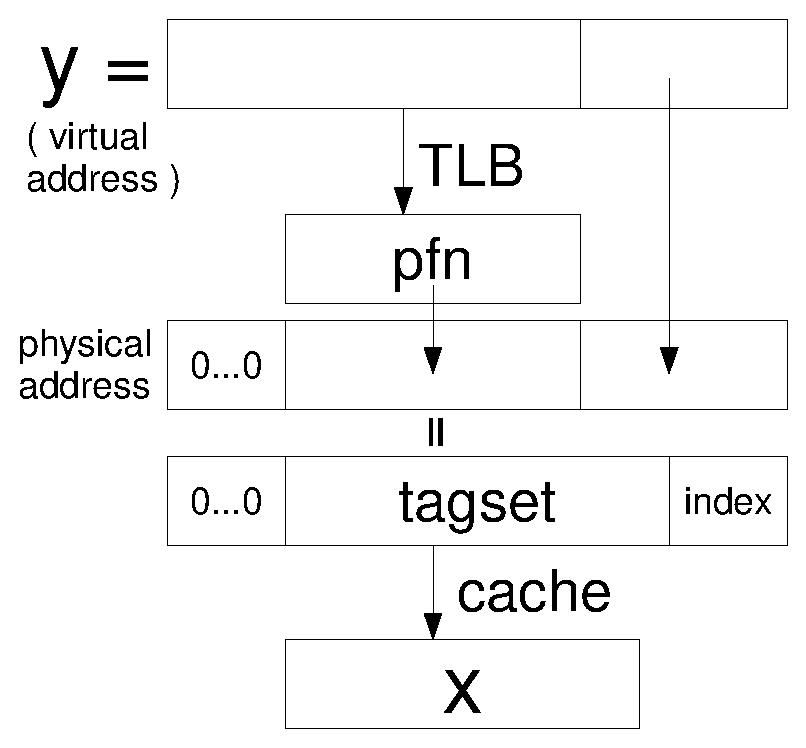
\includegraphics[width=0.4\textwidth]{load}
\caption{Model of LOAD/STORE instructions.}
\end{figure} %\\ \noindent

\subsection{Tagsets}

\emph{Tagset} is bit-field of physical address (see pic.~\ref{LOAD}). Each LOAD/STORE instruction has a tagset. Tagset is used by memory management unit for cache access.
\emph{Displacing tagset} is tagset of instruction with l1Miss test situation. \emph{Hit tagset} is tagset of instruction with l1Hit test situation.

The following syntax will be used for operations on tagsets and virtual addresses:
\begin{enumerate}
\item "bit-extraction" $x_{<5>}$ is the 5th bit of $x$;
\item "bit-range-extraction" $x_{<5..3>}$ is bits from 5th to 3th of $x$;
\item "bit-concatenation" $x||y$.
\end{enumerate}

\subsection{Satisfiability Modulo Theories}
SMT (Satisfiability Modulo Theories) problem is "the satisfiability
problem of the quantifier-free fragment of various first-order
theories"~\cite{SMT}. SMT-solvers concern SMT problem as SAT problem
(satisfiability) with special terms. Conjunctions of these terms can
be satisfied by special algorithms and heuristics. Examples of
SMT-solvers are Yices~\cite{Yices}, Z3~\cite{Z3}, CVC3~\cite{CVC3}.
This article uses bit-vector theory for constraints described
tagsets and registers values relations.

\subsection{Limitations of the approach}
There are some requirements to the testing process which are took into account and efficiently used in proposing approach.
\begin{enumerate}
\item known initial state of the cache and TLB; this is a key requirement of the approach; initial state is used for initial values of registers generation;
\item hits in Joint TLB are considered only; misses (i.e., absence a TLB line for virtual address) requires hardware or software refilling programs, so this test situations are very hard for constraints definition;
\item `Cached Mapped' segments of virtual memory only; another segments may require more complex constraints because of number of cases growth;
\item L1 cache only; L2 cache can contain data and instructions; so cache with only type of contents is considered.
\end{enumerate}

\section{Test case generation}

Test case is a test program. Each test program consists of initialization instructions, body instructions and finalization instructions. Initialization instruction prepare microprocessor to the appropriate state. Then body instructions are executed (they are defined in test template). And finalization instructions check state of microprocessor after body instructions execution (for example, check values for registers).

The aim of proposing algorithm is generation initial values for registers using solution of SMT-constraints. Generated initial values are used for initialization instructions generation. SMT-constraints describe relations on registers values. Each instruction can change values of registers and cache state. Additional variables should be introduced to describe changes of cache state. These variables are tagsets. They don't present cache as it is (by cells). Instead of this constraints on tagsets describe relations between virtual addresses of instructions. Registers are used to get virtual addresses (as second arguments of LOAD and STORE) and values loaded or stored to memory (as first arguments of LOAD and STORE).

The following constraints present cache behavior for \emph{simple} test templates only, i.e. templates with no more than $w+1$ misses (and unlimited count of hits). $w$ is associativity of cache.

\subsection{Tagsets constraints}
Lets $L$ is set of all tagsets from initial cache state and $PFN$ is
set of all physical frame number fields of TLB lines from initial
TLB state. Lets $LP = \{ x | x \in L \wedge x_{<pfn~bits>} \in
PFN\}$. Then walk through given test template and collect
constraints from test situations by the following way:
\begin{enumerate} \item for "l1Hit($x$)": $x \in LP \cup \{ x_1,
..., x_n \}$, where $x_1, ..., x_n$ are all previous displacing
tagsets; algorithm returns "no solution"\ , if $LP \cup \{ x_1, ...,
x_n \} = \varnothing$; \item for "l1Miss($x$)": $x \notin \{x_1,
..., x_n \} \wedge (x \notin LP \vee \bigvee_{\lambda \in LP} (x =
\lambda \wedge LRU(\lambda, x_1, ..., x_n))$, where $x_1, ..., x_n$
are all previous displacing tagsets. \end{enumerate}

Constraint $LRU(\lambda, x_1, ..., x_n) = \bigvee_{\{y_1, ..., y_m\} \subseteq \{x_1, ..., x_n\}} \bigwedge_{t \in \{x_1, ..., y_m\}}  TS(t, \lambda, x_1, ..., x_n,\\y_1, ..., y_m)$, where $\lambda = \lambda_m$ ($m$ is a number of $\lambda$ in its set, $\lambda_1$ is the youngest element of set by LRU order). Constraint $TS$ is the following:\\
$TS(t, \lambda, x_1, ..., x_n, y_1, ..., y_m) = \\
\begin{cases}
R(t) \neq R(\lambda),&\text{if~} t:\text{l1Miss} \wedge t \notin \{y_1, ..., y_m\}\\
R(t) = R(\lambda),&\text{if~} t:\text{l1Miss} \wedge t \in \{y_1, ..., y_m\}\\
t \notin \{\lambda_{m+1}, ..., \lambda_w\},&\text{if~} t:\text{l1Hit} \wedge t = x_i \wedge y_1 = x_j \wedge i < j\\
t \in \{\lambda_{m+1}, ..., \lambda_w\}&\text{if~} t:\text{l1Hit} \wedge t = y_p\\ \setminus\{y_1, ..., y_p\},\\
t \notin \{\lambda_{m+1}, ..., \lambda_w\}&\text{if~} t:\text{l1Hit} \wedge t = x_i \wedge x_i \notin \{y_1, ..., y_m\}\\ \setminus\{y_1, ..., y_p\},& \wedge~y_p = x_j \wedge y_{p+1} = x_{j'} \wedge y_m = x_q\\& \wedge~j < i < j' \wedge i < q \\
\end{cases}$

$t$ : l1Hit (or l1Miss) means corresponded test situation of instruction with tagset $t$.

Constraint $LRU(\lambda, x_1, ..., x_n)$ has other representation using \emph{usefulness predicates}. Tagset is \emph{useful}, if it helps to displace tagset $\lambda$ (otherwords, if it does this tagset more older by means of LRU). Constraint $LRU(\lambda, x_1, ..., x_n)$ is satisfied, if tagset $\lambda$ is displaced before current instruction (and current instruction uses $\lambda$ as displacing tagset). So constraint $LRU$ requires all tagsets \textbf{before the closest cache miss before current instruction}, hit tagsets and displacing tagsets. So, this constraint can be represented as follows:
$LRU(\lambda, x_1, ..., x_n) = (\sum u(x_i) \geqslant w-m)$, where $x_i$ is a tagset (not only displacing tagset) before the closest cache miss before the current instruction, $m$ is a number of $\lambda$ in its set, $w$ is set size (i.e., cache associativity), and $u(x_i)$ is a usefulness predicate for $x_i$. Usefulness predicates can be represented as follows: $u(x_i) = (x_i \in \{ \lambda_{m+1}, \lambda_{m+2}, ..., \lambda_w \} \wedge x_i \notin hit~tagsets~from~\{x_1, ..., x_{i-1} \})$, if $x_i$ is hit tagset, and $u(x_i) = (R(x_i) = R(\lambda))$, if $x_i$ is displacing tagset. This representation is simpler but requires linear inequalities support in solver.

These constraints describe cache behavior without exponential selection all values of any variable. And often $LP$ is not large. Proposed algorithm is correct, full and defines fast way to get tagsets.

\subsection{Register constraints}
Additional constraints should be extracted from test template
($TsLen$ is bit-length of tagsets, $PfnLen$ is bit-length of
physical frame number field of TLB line, $OfsLen$ is offset
bit-length of virtual address):

\begin{enumerate}

\item low bits of tagset equal to the high bits of virtual address's offset for each
instruction "LOAD/STORE $x, y$" with tagset $ts$:
$ts_{<TsLen-PfnLen-1..0>} = y_{<OfsLen-1..OfsLen-TsLen+PfnLen+1>}$;

\item high bits of virtual address correspond to high bits of tagset
(physical frame number bits) for each instruction "LOAD/STORE $x,
y$" with tagset $ts$; these constraints depend on TLB structure; for
example, $y_{<range~bits>} = line.r \wedge y_{<vpn~bits>} =
line.vpn$, where $line$ is TLB line with $line.pfn =
ts_{<TsLen-1~..~TsLen-PfnLen>}$;

\item high bits of virtual address correspond to the segment of virtual memory;

\item for each pair "STORE $x_1, y_1$"
and "LOAD $x_2, y_2$" (LOAD follows from STORE) $phys_1 = phys_2
\wedge phys_1 \notin P \rightarrow x_1 = x_2$, where $phys_i = ts_i
|| {y_i}_{<OfsLen-TsLen+PfnLen..0>}$ (physical addresses), $i \in
\{1, 2\}$, $P$ is set of physical addresses of STORE instructions
between these "STORE" and "LOAD" instructions;

\item for each pair "LOAD
$x_1, y_1$" and "LOAD $x_2, y_2$" (the second LOAD follows from the
first LOAD) $phys_1 = phys_2 \wedge phys_1 \notin P \rightarrow x_1
= x_2$, where $phys_i = ts_i || {y_i}_{<OfsLen-TsLen+PfnLen~..~0>}$
(physical addresses), $i \in \{1, 2\}$, $P$ is set of physical
addresses of STORE instructions between these "LOAD" instructions.
\end{enumerate}

\subsection{SMT representation of constraints}
All generated constraints can be (and should be) represented by constraints on bit-vectors (using bit-extraction and equality relation) and efficiently solved by SMT-solver (we use Yices). $LRU$ constraint was represented using usefulness predicates.

\section{Conclusions}
The article has presented the algorithm for generation test programs used in cache-memory testing. The algorithm works well for simple test templates, i.e. test templates with no more than $w+1$ instructions with cache misses ($w$ is associativity of cache). Further it is planned to increase the algorithm for test situations with uncached or unmapped access and add possibility to offer changes of cache-memory before test program execution to cover more test templates.


\bibliographystyle{latex8}
\bibliography{ksmt}

\end{document}
